\chapter{Results}
In the following chapter the result of physics through spherical decomposition will
be discussed and performance testing will be presented.

\section{Performance}
Since different shaders are impacted differently by different problems a few performance
test-series has been performed and will be discussed below.
For all tests the objects being approximated
are dropped into a bin consisting of static particles. For the complete data collected and
settings used see appendix~\ref{app:test}.

The times presented for velocity and impulse
are the total time for all ten iterations. For the method, the shapes of the objects
 do not affect the simulation significantly and simple boxes have been used in all tests, with one exception.
 In the last test series a Utah Teapot has been voxelized for a more comparable
 test against Bullet 2.83 with a decomposed Utah Teapot.

\subsection{Increasing number of particles per body}
Increasingly fine decomposition lead to more particles per body.
For this test the number of particles per body increase for each series and is
compensated by adding fewer bodies so that the number of particles in the system
in total is kept constant. For all three series some particles from the bin had to be
either added or removed to keep the total equal between the tests.
\begin{figure}[H]
  \centering
  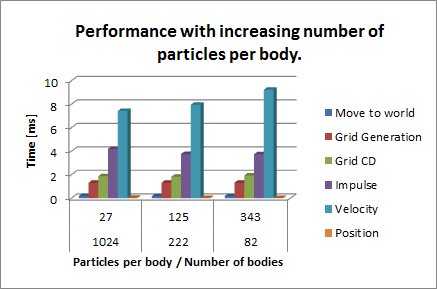
\includegraphics[width = 0.8\textwidth]{particlePerBody2.png}
  \caption{Chart of performance of each of the shader steps for increasing number of particles per body.}
  \label{fig:particlePerBody}
\end{figure}
As we can see the velocity shader time increase with the number of particles
within a body. This is not surprising as the shader performs a gather scheme for
summation of the impulses. The shader will perform a number of global reads proportional
against the number of particles in the body per thread.

\subsection{Increasing number of static particles}
For this test we let the number of static particles in the simulation increase
by increasing the dimensions of the bin.

\begin{figure}[H]
  \centering
  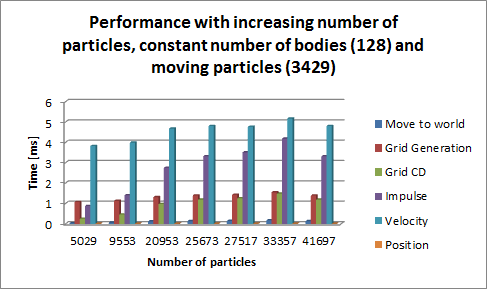
\includegraphics[width = 0.8\textwidth]{staticParticlesIncrease.png}
  \caption{Chart of performance of each of the shader steps for increasing number of static particles.}
\end{figure}

We see some time increase in the grid collision detection and the impulse calculations
and a small increase in the grid generation.
The increase in impulse is not surprising as each particle, even static ones, perform
global reads and writes per particle in the impulse shader step. One could potentially
use a early exit strategy and not perform the impulse calculations for static particles,
however, unless the whole workgroup is static particles one is not guaranteed
any performance gain as returning threads within a workgroup do not ensure
that new work can be performed.

\subsection{Increasing number of bodies and dynamic particles}
For this test we increase both the number of bodies and particles in the system.
\begin{figure}[H]
  \centering
  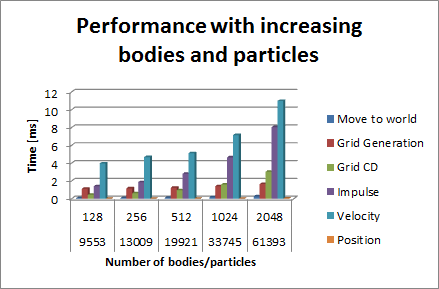
\includegraphics[width = 0.8\textwidth]{bodiesIncrease.png}
  \caption{Chart of performance of each of the shader steps for increasing number of bodies and particles.}
\end{figure}

Here we can see an increase in every shader step.
Worst scaling can be seen among the impulse and velocity step. Those shader steps are the two involved
in the stabilization loop and both are executed ten times each per update and optimizations
to these two steps should be prioritized in the future.

\subsection{Increasing grid size}
This test measures the performance of the grid size. For a M-by-M-by-M grid we can detect collisions
effectively on coordinates between -M/2 and +M/2 in each dimension.
\subsection{Increasing number of bodies and dynamic particles}
For this test we increase the number of bodies (and particles) in the system.
\begin{figure}[H]
  \centering
  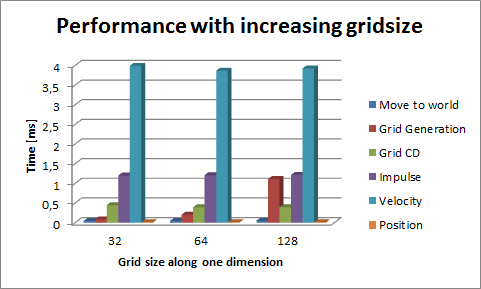
\includegraphics[width = 0.8\textwidth]{gridIncrease.png}
  \caption{Chart of performance of each of the shader steps for increasing number of cells in grid}
\end{figure}

We see that the grid generation scales poorly with the grid size, most likely cubicly
as the number of grid cells increase cubicly and the generation includes the prefix sum and sorting.
We can also note that the grid collision detection does not increase, this is expected since
we still read an equal amount of particles no matter the grid size and the particles are
sorted from the grid generation shader.

\subsection{Increasing cell size}
For this test we increase the size of the simulation domain by increasing the cell size instead.
This leads to more candidate particles, needing to be validated as collisions or not,
as more and more will end up in
the larger and larger surrounding cells.
\begin{figure}[H]
  \centering
  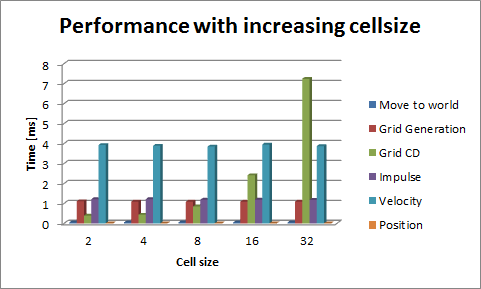
\includegraphics[width = 0.8\textwidth]{cellIncrease.png}
  \caption{Chart of performance of each of the shader steps for increasing cell size}
\end{figure}

It is only the grid collision detection shader which takes a penalty to performances
while changing the cell size, as expected. Note however that for each new series
in this test we get two times the size of the simulation domain in each dimension.
Also note that the time increase from cell size 2 to cell size 8 is only 0.34 ms in total for all shader steps.
This is cheaper than increasing the grid size from 32 to 128, which gives an increase of 0.93 ms.

\subsection{Modified Normals}
While difficult to say wether the end result is more or less physically correct
what can be tested is the amount of stabilization iterations for which the simulation
is still stable (i.e. avoids tunneling). The testing was performed on 5 by 5 by 5
cubes so a decent amount of particles would have modified normals. Without modified
normals at 6 iterations there was severe tunneling between the objects. With replaced normals
 as low as 4 iterations gave no tunneling. In addition when going lower
 and tunneling do occur, with modified normals we have a greater chance of the
 situation resolving itself since the edge particles will always push to separate
 the objects, much as the signed distance field described by~\cite{flex}.
 With weighted normals, as described in section~\ref{sec:modnorm}, some improvement
 could be seen and as few as 6 iterations could be used without tunneling.

\subsection{Tighter voxelization}
Tighter voxelization led to better collision result since the surface is modeled
more accurately, in addition one could decrease the number of iterations needed
for tunnel prevention and stability. This is most likely due to the reduce depth
of the indentations between particles which lead to the normals and resulting forces more often
being directed outwards from the object with a lesser angle.
 With deep indentations between particles the forces will angled more steeply and
  some of the force will not be used for separating the objects.
This method will take a penalty to the collision detection shader step in
terms of performance since many of the bodies own particles will register as collisions
for the tighter voxelization. During testing the benefit of lowering the number of
stabilization iterations greatly outweighed the extra time needed in the collision
detection. Again testing on the 5 by 5 by 5 cubes without tightened voxelization 6 iterations resulted in
tunneling, with tightened voxelization as low as 3 iterations still managed without tunneling.

\subsection{Voxelized Teapot}\label{sec:teapot}
For this final test a Utah Teapot has been voxelized into 171 spheres, see figure~\ref{fig:voxteapot}.
The testing constist of two test series. One with 256 bodies and one with 512 bodies.
Each setup tested with 10 and 5 stabilization iterations. These results can be compared to the
results from Bullet in chapter~\ref{sec:hacd} and are therefore included in the graphs.

\begin{figure}[H]
  \centering
  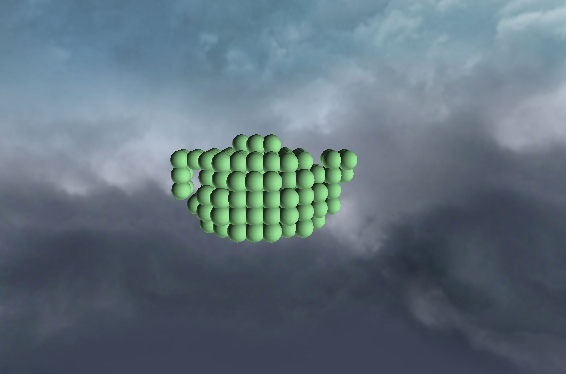
\includegraphics[width = 0.8\textwidth]{voxteapot.png}
  \caption{Teapot voxelized with 171 spheres}
  \label{fig:voxteapot}
\end{figure}


At 512 bodies and 5 iterations spherical voxelization see a speedup of a factor of 2 compared to
Bullet with no sleeping. At 10 iterations a speedup of a factor of 1.3.
When Bullets' sleeping is activated it's slower than spherical voxelization at 5 stabilization iterations but faster than
spherical voxelization at 10 stabilization iterations. See figure~\ref{fig:GvC512}.

\begin{figure}[H]
  \centering
  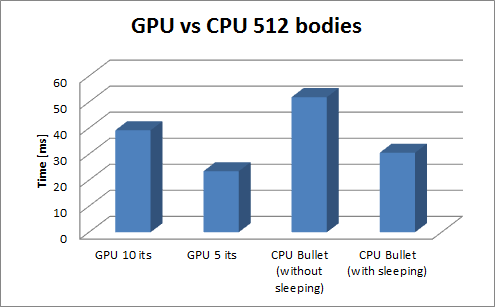
\includegraphics[width = 0.8\textwidth]{graphs/GvC512.png}
  \caption{Chart of performance comparison between spherical voxelization and Bullet for 512 bodies}
  \label{fig:GvC512}
\end{figure}

At 256 bodies the speedup is not as large. Comparing 5 stabilization iterations on the
GPU solution to Bullet without sleeping gives a speedup with a factor of 1.6.
At 10 stabilization iterations spherical voxelization is somewhat slower than Bullet.
With sleeping enabled Bullet is faster than the GPU solution at 5 stabilization iterations, even if
only by a small margin. See figure~\ref{fig:GvC256}

\begin{figure}[H]
  \centering
  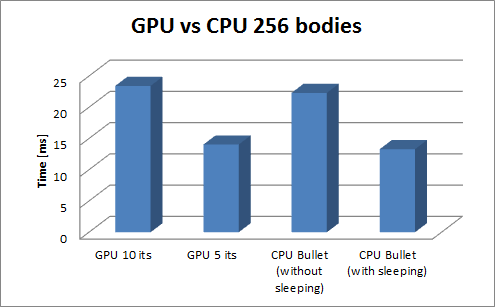
\includegraphics[width = 0.8\textwidth]{graphs/GvC256.png}
  \caption{Chart of performance comparison between spherical voxelization and Bullet for 256 bodies}
  \label{fig:GvC256}
\end{figure}

\section{Limitations}
\subsection{Per body particle limit}
Currently in the velocity update shader there is a for-loop across all the spheres
belonging to the current body, this is done to gather all the forces from the spheres.
To ensure performance on the GPU one uses unrolling, i.e. the for-loops content is
duplicated for as many iterations as necessary. However on the GPU this mean two
things, we have trouble with dynamic length on the for-loops and there is a upper
bound on the number of iterations that are allowed. For the hardware used for the thesis,
this limit is 4096. Therefor the method is currently limited to a maximum of 4096
spheres per body.

\subsection{Tunneling}
Tunneling can occur in the system as no protection against the phenomenon is implemented.
For linear movement such a protection is easily implemented, however with rotations
the protection is slightly more difficult to implement properly. For long thin
objects a smaller time step is recommended.
\subsection{Limited domain}
In addition the domain of the simulation has to be determined before the simulation start
as a uniform spatial partitioning grid is used for the collision detection.

\subsection{False alignment}
Since the method uses spheres as a principal shape the result has a tendency to align
with the grid. A single box consisting of 27 sphere fall on a plane, also made up of spheres
at a slight rotation. All impulses present will drift towards the cube aligning with the
plane at intervals of 90 degrees. The effect would be less apparent with less regularly shaped objects and
is remedied somewhat by friction, albeit not completely.

\section{Comparison to bullet}
\subsection{Concavity}
The method can handle concavity through spherical decomposition. The detail of of
the resulting collision shape is highly dependent on voxelization resolution.
Since the collision detection is designed to operate on spheres of equal size
objects such as the Utah teapot with both large and small features can quickly get
a high number of spheres. HACD can model these with a single larger hull for the body
and smaller hulls for the smaller features.

\subsection{Performance}
In section~\ref{sec:teapot} we see that when simulating many rigid bodies spherical
voxelization shows an improvement in performance over Bullet. However increasing
the detail in the decomposition will quickly reduce the performance.

Since the velocity and impulse shader steps are iterated
several times for stabilization these steps are quite vital to the performance
of the method. More work could be spent on improving the performance of these shaders,
but one should also investigate if the stabilization iterations could be exchanged for
shock propagation. As already shown by the results achieved by~\cite{flex} with nVidia Flex.

\subsection{Correctness}
Correctness for spherical decomposition depend highly on how finely the model is
decomposed, much like how Bullet's HACD depends on how many vertices are allowed
per model and how many models are used. Boxes with as low as 27 particles looks convincing, but e.g. a Utah Teapot
may need many more particles to produce convincing results, at 171 particles the
Utah teapot looks decently decomposed.
